\documentclass[10pt]{beamer}
\usepackage[utf8]{inputenc}
\usepackage[T1]{fontenc}
\usepackage[french]{babel}
\usepackage{amsmath,minted,amsfonts,amssymb,tikz,graphicx,geometry,tkz-tab,pgfplots,float}
\usemintedstyle{tango}
\usetheme[hideallsubsections]{UPPA2014}
\title{Projet POO, Dashboard}
\author{Romane Sallio \and Pierre Fontaine}
\institute{UPPA, Licence, Informatique}

\begin{document}

\begin{frame}
  \titlepage
\end{frame}

\begin{frame}
  \frametitle{Sommaire}
  \tableofcontents
\end{frame}

\section{introduction}

\begin{frame}
  \frametitle{Introduction}
  %\framesubtitle{Sous titre: objet}
  Dashboard est le projet que nous avons conçu en C++ avec le paradigme Objet.

  Nous avons utilisé le Framework QT pour développer l'interface utilisateur.

  Son objectif est simple : permettre à l'utilisateur d'avoir les éléments essentiels à porté de click.
\end{frame}

\section{Pourquoi QT}
\subsection{Des classes}
\begin{frame}
  \frametitle{Pourquoi QT}
  \framesubtitle{Paradigme Objet}
  QT est écrit en C++ et est implémenté selon le paradigme objet. Chacun des composants réfère à une classe particulière qui peut ou non dérivé d'une autre classe mère.
\end{frame}
  \subsection{JS Like}
    \begin{frame}
      \frametitle{Pourquoi QT}
      \framesubtitle{JS LIKE}
      Lors de l'utilisation d'un nouveau \emph{Framework}, une partie crucial du temps est concacré à l'étude du fonctionnement de celui ci. Il semblait évident qu'après avoir étudier le \emph{JavaScript}, le \emph{QT} qui partage la même philosophie de la gestion d'évènement \emph{(Async/Sync)} serait plus digeste.
    \end{frame}
\section{Spécifications techniques du code}
\subsection{Template}

\begin{frame}
  \frametitle{Template}
  \framesubtitle{Utilité ?}
  La technique consiste à paramétrer le Type. Ainsi l'utilisateur de la classe pourra utiliser le type \emph{int, shorting, string ...}.\\

  Utilisé dans \emph{List.h}\\

  Pourquoi ?
  \begin{enumerate}
    \item Créer une liste de n'importe quoi
    \item Container important
  \end{enumerate}

  \begin{alertblock}{attention}
    L'implémentation ne peut être séparée de la signature.
  \end{alertblock}
\end{frame}

\begin{frame}[fragile]
  \frametitle{Template}
  \framesubtitle{Code}
  \begin{minted}{c++}
template <class T>
class List{...};
  \end{minted}
\end{frame}

  \subsection{Forme canonique de coplien}
\begin{frame}[fragile]
  \frametitle{Forme canonique de coplien}
  \framesubtitle{Pourquoi}

  Il est interressant dans la conception de \emph{container} comme des listes, des sets ... qu'ils puissent s'affecter entre eux, se construire à partir d'un modèle déjà existant.\\

  C'est pourquoi nous intégrons ce modèle dans quelques classes comme :
  \begin{enumerate}
    \item list.h
    \item abstractmesureunite.h
  \end{enumerate}
\end{frame}

\begin{frame}[fragile]
  \frametitle{Forme canonique de coplien}
  \framesubtitle{code 1}

  \begin{minted}{cpp}
class AbstractMesureUnite{
protected:
  double _value;
public:
  AbstractMesureUnite();
  AbstractMesureUnite(double);
  AbstractMesureUnite(const AbstractMesureUnite&);
  ~AbstractMesureUnite();
  AbstractMesureUnite &operator=(const AbstractMesureUnite&);
  ...
};
  \end{minted}
\end{frame}

\begin{frame}[fragile]
  \frametitle{Forme canonique de coplien}
  \framesubtitle{code 2}

  \begin{minted}{cpp}
template <class T>
class List{
protected:
    struct cellule{
        cellule *suivant;
        T valeur;
    };
    typedef cellule* liste;
    liste _l;
public:
    List();
    ~List();
    List(const List<T> &l);
    List<T> operator=(const List<T>);
    ...
};
  \end{minted}
\end{frame}

\subsection{Classe Abstraite}
\begin{frame}
  \frametitle{Classe Abstraite}
  \framesubtitle{Interet}
  \structure{Factorisation du code :}

  L'un des objectifs majeur lorsque l'on developpe du code c'est de s'assurer qu'on ne se répetera pas.\\

  \structure{Creer une signature que l'on implémente pas :}

  \begin{enumerate}
    \item les sous classes fourniront l'implémenteront forcément
    \item les sous classes auront chacune une implémentation différente.
    \item cette classe abstraite ne sera jamais instancié.
  \end{enumerate}
\end{frame}

\begin{frame}
  \frametitle{Classe Abstraite}
  \framesubtitle{QT}
  \begin{center}
    \begin{figure}
      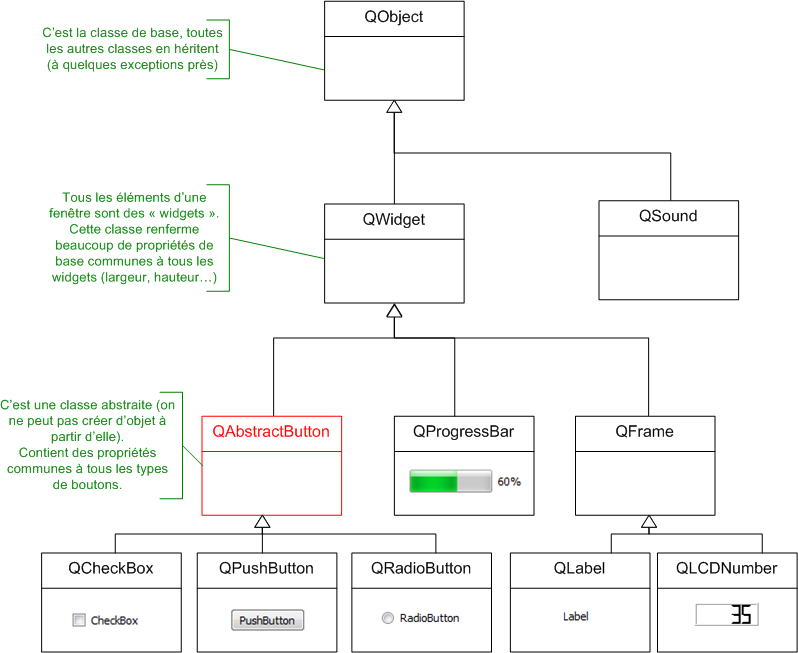
\includegraphics[scale=0.3]{img/qtUml.png}
      \caption{Qt Diagram openclassroom}
    \end{figure}
  \end{center}
\end{frame}

\begin{frame}[fragile]
  \frametitle{Classe Abstraite}
  \framesubtitle{Code 1}
  \begin{minted}[breaklines]{cpp}
class AbstractMesureUnite{
protected:
  double _value;
public:
  AbstractMesureUnite();
  AbstractMesureUnite(double);
  AbstractMesureUnite(const AbstractMesureUnite&);
  ~AbstractMesureUnite();
  AbstractMesureUnite &operator=(const AbstractMesureUnite&);
  ...
  virtual void afficher(ostream &flux) const = 0;

  friend ostream& operator<<(ostream& flux,const AbstractMesureUnite& u){
    u.afficher(flux);
    return flux;
  }
};
  \end{minted}
\end{frame}
\begin{frame}[fragile]
  \frametitle{Classe Abstraite}
  \framesubtitle{Code 2}
  \begin{minted}[breaklines]{cpp}
class Temperature : public AbstractMesureUnite{
public:
  Temperature();
  Temperature(double);
  virtual void afficher(ostream &flux) const = 0;
  virtual double getCelsius()const = 0;
  virtual double getFahrenheit()const = 0;
  virtual double getKelvin()const = 0;
};
  \end{minted}
\end{frame}

  \subsection{Heritage}
\begin{frame}
  \frametitle{Heritage}
  \framesubtitle{QT}
  \structure{Dérivation des composants :}

  \begin{enumerate}
    \item Chaque composant du framework QT est une classe
    \item Créer un composant spécifique se fait en dérivant un composant général
  \end{enumerate}
  \begin{block}{tips}
    Il est courant que les classes les plus généralistes ne soient pas instanciables, ce sont des classes \emph{abstraites}.
  \end{block}
\end{frame}

\begin{frame}[fragile]
  \frametitle{Heritage}
  \framesubtitle{Hériter un composant QT}

  \begin{minted}[breaklines]{cpp}
#include <QWidget>

class Module : public QWidget{
    Q_OBJECT
protected:
  //méthodes protégées.
public:
  explicit Module(QWidget *parent = 0,double h = 300, double w = 400);
  //méthodes publiques

signals:
  //signals
public slots:
  //slots
};
  \end{minted}
\end{frame}

\begin{frame}[fragile]
  \frametitle{Heritage}
  \framesubtitle{En dehors de QT}
  \begin{center}
    \begin{figure}
      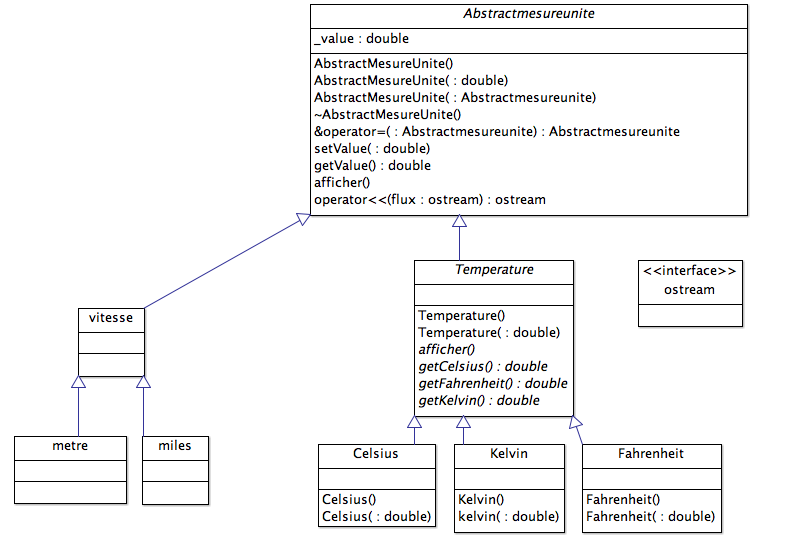
\includegraphics[scale=0.4]{img/Diagrammedeclasses.png}
    \end{figure}
  \end{center}
\end{frame}

  \subsection{Classe Complexe}
\begin{frame}
  \frametitle{Classe Complexe}
  \framesubtitle{interet ?}
  \structure{Concept :}

  Une classe peut utiliser l'instance d'une autre classe.\\
  \structure{Exemple d'une vue :}

  Prenons pour exemple notre \emph{widget Météo}. Celui ci a besoin d'afficher des informations, donc qui fournit l'information ?

  On instancie une classe \emph{Meteodata} qui va servir d'intermediaire entre la vue et le modèle.
\end{frame}

\begin{frame}[fragile]
  \frametitle{Classe Complexe}
  \framesubtitle{code}
  \begin{minted}[breaklines]{cpp}
class MeteoJour : public QWidget{
    Q_OBJECT
protected:
    ...
    //model
    MeteoData *_data;
public:
    explicit MeteoJour(int j,MeteoData *data,QWidget *parent = 0);
signals:
    ...
public slots:
    ...
};
  \end{minted}
\end{frame}

\section{conclusion}
\begin{frame}
\frametitle{Conclusion}
  \begin{itemize}
    \item code plus facile à gérer en collaboration
    \item code plus facile à maintenir
    \item évolution envisageable
    \item ré-utilisation de code
    \item plus efficace pour IHM
  \end{itemize}
\end{frame}
\end{document}
